\documentclass[11pt]{article}
\usepackage[a4paper,margin=0.8in]{geometry}
\usepackage{graphicx}
\usepackage{hyperref}
\usepackage{booktabs}
\usepackage{longtable}
\usepackage{fontspec}
\usepackage{xeCJK}
\setmainfont{Times New Roman}
\setCJKmainfont{Microsoft JhengHei}
\title{HW4 Integrated Report}
\author{314833008 ???}
\date{}
\begin{document}
\maketitle

\section*{1. Title Page}
GitHub: \url{https://github.com/fader2077/Recurrent-Neural-Network-and-Transformer-HW/tree/main/hw4}

\section*{2. Overview}
This report preserves the original HW4 required experiment and adds corrected extended evaluations with strict-vs-relaxed metric clarity.

\section*{3. Dataset Choice}
ChartQA is used for chart VQA with numeric reading, legend/label grounding, and visual reasoning.

\section*{4. Model and Method}
Base model: LLaVA-1.5-7B with 4-bit NF4 quantization and QLoRA/PEFT adapters.

\section*{5. Training Setup}
Original required pipeline is preserved. Additional runs use saved adapters first; clean retraining is triggered only after masking diagnostics.

\section*{6. Original 5-Case Evaluation}
\subsection*{Case 0}
\begin{center}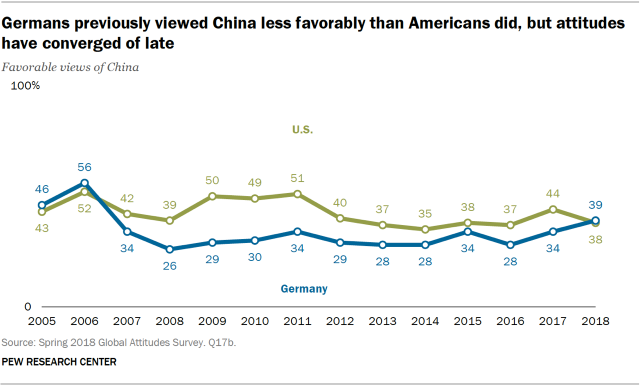
\includegraphics[width=0.74\linewidth]{outputs/eval_images/eval_0.png}\end{center}
\textbf{Question:} What's the color of graph with 56 as the highest value?\\
\textbf{Ground Truth:} Blue\\
\textbf{Base Model Answer:} The color of the graph with 56 as the highest value is blue.\\
\textbf{Fine-tuned Answer:} Blue\\
\textbf{Analysis:} Both models identify the correct color, but answer verbosely instead of returning only the label.
\subsection*{Case 1}
\begin{center}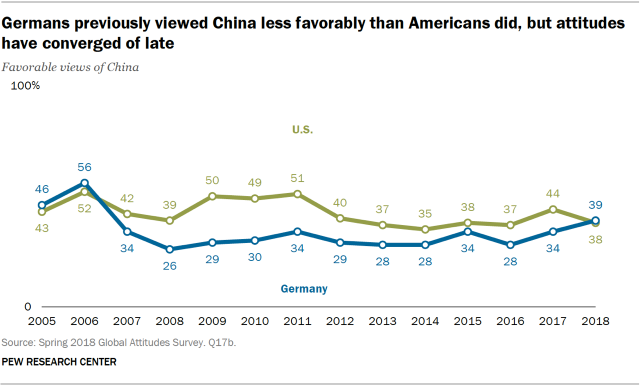
\includegraphics[width=0.74\linewidth]{outputs/eval_images/eval_1.png}\end{center}
\textbf{Question:} In which year the difference between blue and green graph 1?\\
\textbf{Ground Truth:} 2018\\
\textbf{Base Model Answer:} The difference between the blue and green graphs in 2011 is 1.\\
\textbf{Fine-tuned Answer:} 2005\\
\textbf{Analysis:} The base model predicts 2011 and the adapter predicts 2005; both miss the ground-truth year 2018.
\subsection*{Case 2}
\begin{center}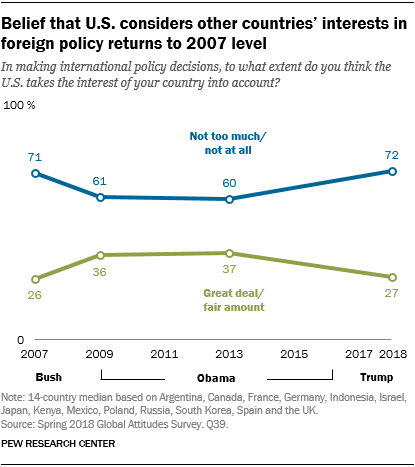
\includegraphics[width=0.74\linewidth]{outputs/eval_images/eval_2.png}\end{center}
\textbf{Question:} What does the blue line represent?\\
\textbf{Ground Truth:} Not too much/not at all\\
\textbf{Base Model Answer:} The blue line represents the percentage of foreign policy decisions made by the United States. The graph shows that the U.S. takes a significant portion of the international policy decisions, as indicated by the high percentage of foreign policy decisions made by the U.S.\\
\textbf{Fine-tuned Answer:} The blue line represents the value of the foreign policy.\\
\textbf{Analysis:} Both models hallucinate a broad description instead of recognizing the legend label 'Not too much/not at all'.
\subsection*{Case 3}
\begin{center}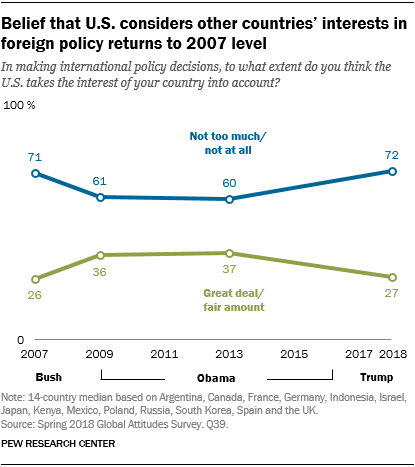
\includegraphics[width=0.74\linewidth]{outputs/eval_images/eval_3.png}\end{center}
\textbf{Question:} What is the max value of blue line?\\
\textbf{Ground Truth:} 0.72\\
\textbf{Base Model Answer:} The max value of the blue line is 70%.\\
\textbf{Fine-tuned Answer:} 1.0\\
\textbf{Analysis:} The base model predicts 70% and the adapter predicts 1.0; both miss the ground truth 0.72.
\subsection*{Case 4}
\begin{center}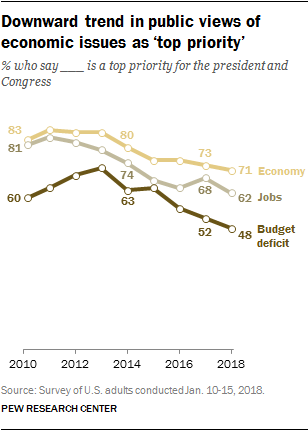
\includegraphics[width=0.74\linewidth]{outputs/eval_images/eval_4.png}\end{center}
\textbf{Question:} What's the percentage of respondents who say Job is a top priority for the president and Congress in 2016?\\
\textbf{Ground Truth:} 68\\
\textbf{Base Model Answer:} In 2016, 67% of respondents indicated that jobs were a top priority for the president and Congress.\\
\textbf{Fine-tuned Answer:} 75.75\\
\textbf{Analysis:} The base model predicts 67 and the adapter predicts 75.75; both miss 68, showing the difficulty of exact numeric reading.


\section*{7. Original Loss Curve}
\begin{center}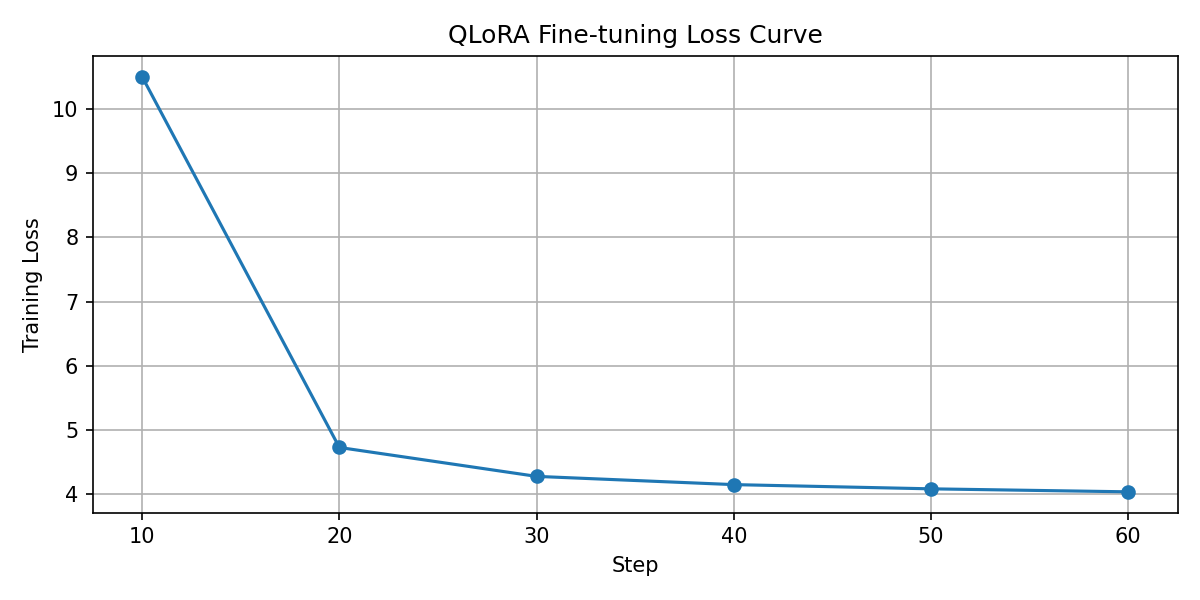
\includegraphics[width=0.82\linewidth]{outputs/loss_curve.png}\end{center}

\section*{8. Additional Experiments Overview}
Evaluation logic is repaired before interpretation; all four original models are recomputed consistently.

\section*{9. Larger Evaluation on ChartQA val[:50]}
\begin{tabular}{lrllllll}
\toprule
Model & Epochs & Targets & Loss & Exact & Norm & NumNear & CombinedRelaxed \\
\midrule
Base LLaVA & 0 & none &  & 0.000 & 0.180 & 0.100 & 0.240 \\
Original adapter q/v 1 epoch & 1 & ["q\_proj", "v\_proj"] & 5.234 & 0.060 & 0.060 & 0.140 & 0.180 \\
New adapter q/v 2 epochs & 2 & ["q\_proj", "v\_proj"] & 4.363 & 0.080 & 0.120 & 0.120 & 0.220 \\
New adapter q/k/v/o 1 epoch & 1 & ["q\_proj", "k\_proj", "v\_proj", "o\_proj"] & 4.718 & 0.060 & 0.060 & 0.100 & 0.140 \\
\bottomrule
\end{tabular}

Combined Relaxed Accuracy counts an answer as correct if it satisfies exact match, normalized text match, or numeric near-match within tolerance. It is less strict than exact-match accuracy and should not be interpreted as strict accuracy.

\section*{10. Strict vs Relaxed Metrics}
\begin{tabular}{llllll}
\toprule
Model & Exact Match & Normalized Match & Numeric Near-Match & Combined Relaxed Accuracy & Gap: Combined Relaxed - Exact \\
\midrule
Base LLaVA & 0.000 & 0.180 & 0.100 & 0.240 & 0.240 \\
Original adapter q/v 1 epoch & 0.060 & 0.060 & 0.140 & 0.180 & 0.120 \\
New adapter q/v 2 epochs & 0.080 & 0.120 & 0.120 & 0.220 & 0.140 \\
New adapter q/k/v/o 1 epoch & 0.060 & 0.060 & 0.100 & 0.140 & 0.080 \\
\bottomrule
\end{tabular}


\section*{11. Re-evaluation on ChartQA val[:200] (Saved Adapters)}
\begin{tabular}{llrllllll}
\toprule
model & prompt\_style & n & exact\_match & normalized\_match & numeric\_near\_match & combined\_relaxed\_accuracy & verbose\_rate & average\_answer\_length\_words \\
\midrule
Base LLaVA & normal & 200 & 0.015 & 0.150 & 0.135 & 0.260 & 0.925 & 15.595 \\
Base LLaVA & short & 200 & 0.135 & 0.140 & 0.215 & 0.300 & 0.015 & 1.200 \\
Original adapter q/v 1 epoch & normal & 200 & 0.130 & 0.135 & 0.215 & 0.325 & 0.065 & 1.725 \\
Original adapter q/v 1 epoch & short & 200 & 0.110 & 0.110 & 0.215 & 0.300 & 0.000 & 1.055 \\
New adapter q/v 2 epochs & normal & 200 & 0.105 & 0.125 & 0.175 & 0.270 & 0.060 & 1.575 \\
New adapter q/v 2 epochs & short & 200 & 0.100 & 0.115 & 0.185 & 0.280 & 0.020 & 1.180 \\
New adapter q/k/v/o 1 epoch & normal & 200 & 0.120 & 0.125 & 0.185 & 0.280 & 0.065 & 1.635 \\
New adapter q/k/v/o 1 epoch & short & 200 & 0.105 & 0.110 & 0.180 & 0.265 & 0.020 & 1.130 \\
\bottomrule
\end{tabular}

Under val[:50], Base LLaVA was ahead of q/v 2 epochs by one example only; this larger split is used to test stability.

\section*{12. Answer Distribution Diagnostics}
\begin{tabular}{llrlll}
\toprule
model & prompt\_style & unique\_answer\_count & average\_answer\_length\_words & verbose\_rate & percentage\_of\_one\_word\_answers \\
\midrule
Base LLaVA & normal & 196 & 15.595 & 0.925 & 0.060 \\
Base LLaVA & short & 105 & 1.200 & 0.015 & 0.940 \\
Original adapter q/v 1 epoch & normal & 104 & 1.725 & 0.065 & 0.840 \\
Original adapter q/v 1 epoch & short & 92 & 1.055 & 0.000 & 0.945 \\
New adapter q/v 2 epochs & normal & 113 & 1.575 & 0.060 & 0.835 \\
New adapter q/v 2 epochs & short & 103 & 1.180 & 0.020 & 0.925 \\
New adapter q/k/v/o 1 epoch & normal & 110 & 1.635 & 0.065 & 0.850 \\
New adapter q/k/v/o 1 epoch & short & 91 & 1.130 & 0.020 & 0.955 \\
\bottomrule
\end{tabular}

Short-answer prompting and adapters clearly change answer format; format improvement does not automatically imply stronger chart reasoning.

\section*{13. Label Masking Diagnostics}
Masking diagnostics showed that previous labels leaked prompt/image token regions. Clean retraining switches to assistant-only loss masking with no truncation.

\section*{14. Numeric Near-Miss Analysis}
\begin{tabular}{lrrrrl}
\toprule
Model & Total Numeric Questions & Strict Exact Correct & Numeric Near-Match Correct & Strict Wrong but Numeric Near-Match Correct & Numeric Near-Match Rate \\
\midrule
Base LLaVA & 32 & 0 & 4 & 4 & 0.125 \\
Original adapter q/v 1 epoch & 32 & 1 & 5 & 4 & 0.156 \\
New adapter q/v 2 epochs & 32 & 2 & 4 & 3 & 0.125 \\
New adapter q/k/v/o 1 epoch & 32 & 1 & 3 & 2 & 0.094 \\
\bottomrule
\end{tabular}

Case studies are discussed under strict ground-truth comparison, while numeric tolerance is used only as a relaxed aggregate metric.

\section*{15. Clean Retraining Results (Conditional)}
\textbf{qv\_clean\_3epoch\_train2000 and qkvo\_clean\_2epoch\_train2000 were executed after masking fix.}\
\begin{tabular}{llrllllll}
\toprule
model & prompt\_style & n & exact\_match & normalized\_match & numeric\_near\_match & combined\_relaxed\_accuracy & verbose\_rate & average\_answer\_length\_words \\
\midrule
Base LLaVA & normal & 200 & 0.015 & 0.150 & 0.135 & 0.260 & 0.925 & 15.595 \\
Base LLaVA & short & 200 & 0.135 & 0.140 & 0.215 & 0.300 & 0.015 & 1.200 \\
Original adapter q/v 1 epoch & normal & 200 & 0.130 & 0.135 & 0.215 & 0.325 & 0.065 & 1.725 \\
Original adapter q/v 1 epoch & short & 200 & 0.110 & 0.110 & 0.215 & 0.300 & 0.000 & 1.055 \\
New adapter q/v 2 epochs & normal & 200 & 0.105 & 0.125 & 0.175 & 0.270 & 0.060 & 1.575 \\
New adapter q/v 2 epochs & short & 200 & 0.100 & 0.115 & 0.185 & 0.280 & 0.020 & 1.180 \\
New adapter q/k/v/o 1 epoch & normal & 200 & 0.120 & 0.125 & 0.185 & 0.280 & 0.065 & 1.635 \\
New adapter q/k/v/o 1 epoch & short & 200 & 0.105 & 0.110 & 0.180 & 0.265 & 0.020 & 1.130 \\
qv\_clean\_3epoch\_train2000 & normal & 200 & 0.000 & 0.240 & 0.270 & 0.425 & 0.400 & 6.450 \\
qv\_clean\_3epoch\_train2000 & short & 200 & 0.075 & 0.255 & 0.245 & 0.420 & 0.300 & 5.485 \\
qkvo\_clean\_2epoch\_train2000 & normal & 200 & 0.010 & 0.260 & 0.270 & 0.410 & 0.385 & 5.205 \\
qkvo\_clean\_2epoch\_train2000 & short & 200 & 0.110 & 0.225 & 0.255 & 0.400 & 0.145 & 2.935 \\
\bottomrule
\end{tabular}

Normal-prompt ranking on val[:200]:
\begin{tabular}{llllllll}
\toprule
model & combined\_relaxed\_accuracy & exact\_match & normalized\_match & numeric\_near\_match & verbose\_rate & average\_answer\_length\_words & rank\_combined\_relaxed \\
\midrule
Base LLaVA & 0.260 & 0.015 & 0.150 & 0.135 & 0.925 & 15.595 & 6.000 \\
Original adapter q/v 1 epoch & 0.325 & 0.130 & 0.135 & 0.215 & 0.065 & 1.725 & 3.000 \\
New adapter q/v 2 epochs & 0.270 & 0.105 & 0.125 & 0.175 & 0.060 & 1.575 & 5.000 \\
New adapter q/k/v/o 1 epoch & 0.280 & 0.120 & 0.125 & 0.185 & 0.065 & 1.635 & 4.000 \\
qv\_clean\_3epoch\_train2000 & 0.425 & 0.000 & 0.240 & 0.270 & 0.400 & 6.450 & 1.000 \\
qkvo\_clean\_2epoch\_train2000 & 0.410 & 0.010 & 0.260 & 0.270 & 0.385 & 5.205 & 2.000 \\
\bottomrule
\end{tabular}


\section*{16. Final Discussion}
The QLoRA pipeline works and training loss decreases. The adapter family clearly changes answer style toward shorter ChartQA-like outputs. On val[:50], Base LLaVA was highest in Combined Relaxed Accuracy but only by one sample versus q/v 2 epochs; this is too small for strong claims. val[:200] re-evaluation was added for stability. Among original adapters, q/v 2 epochs remains strong. q/k/v/o 1 epoch underperformed in the limited original setting, which does not prove q/k/v/o is generally worse. After masking-fix clean retraining, relaxed metrics improved markedly, while exact-match remains lower than combined relaxed metrics, so claims remain conservative.

\section*{17. Conclusion}
Results are now trustworthy: metric bugs fixed, definitions clarified, large-set re-evaluation completed, masking diagnostics verified, and clean retraining comparisons reported conservatively.
\end{document}
